\section{Produktfunktionen}
	% \input{3-Produktfunktionen}

		\subsection{Use Cases}
		% \input{3-1-Use_Cases}
		
		In dem zu modellierenden System gibt es zwei Unterumgebungen (\emph{Server} sowie \emph{Robot Unit}), auf welchen die Aktoren \emph{Customer}, \emph{Hospital} und \emph{Robot Unit} verschiedene Anwendungsfälle aufrufen können. Der fiktionale Aktor \emph{User} aggregiert die gemeinsamen Use-Cases von \emph{Customer} und \emph{Hospital} \\
		Die Abbildungen \ref{fig:3-1-server-use-cases} und \ref{fig:3-1-use-cases-robot-unit} stellen die Funktionalitäten dieser Teilsysteme dar.
			\begin{figure}[H]
				\centering
				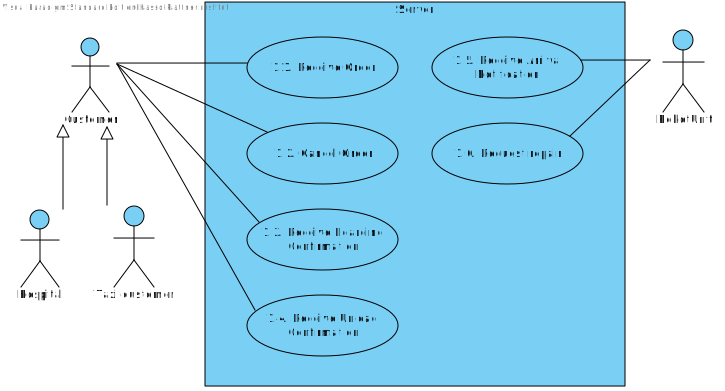
\includegraphics[width=0.8\textwidth]{img/2-Analyse-Server}
				\caption{Use Case Diagramm 1: Use Cases des Teilsystems \emph{Server}}
				\label{fig:3-1-server-use-cases}
			\end{figure}
			
			\begin{figure}[H]
				\centering
				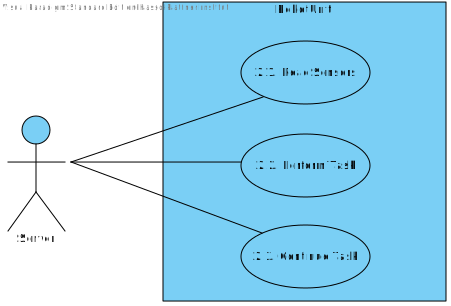
\includegraphics[width=0.8\textwidth]{img/2-Analyse-RobotUnit}
				\caption{Use Case Diagramm 2: Use Cases des Teilsystems \emph{Robot}}
				\label{fig:3-1-use-cases-robot-unit}
			\end{figure}

		\pagebreak


		\subsection{Beschreibung zu Use Case \emph{3}: Read Sensors}

			\subsubsection*{Charakterisierende Informationen}

			\begin{table}[H]
				\centering
				\begin{tabularx}{\textwidth}{|p{5cm}|X|}
				\hline
				\textbf{Übergeordneter elementarer Geschäftsprozess:} & Choose Robot\\ \hline
				\textbf{Ziel des Use Cases:} & \emph{Robot} kann über seinen Akkustand und seine Position Auskunft geben\\ \hline
				\textbf{Umgebende Systemgrenze:} & \emph{Robot} \\ \hline
				\textbf{Vorbedingung:} & \emph{Robot} hat eine Anfrage vom \emph{Server} erhalten \\ \hline
				\textbf{Nachbedingung bei erfolgreicher Ausführung:} & \emph{Robot} schickt die ermittelten Informationen an den \emph{Server} \\ \hline
				\textbf{Beteiligte Nutzer:} & \emph{Robot} \\ \hline
				\textbf{Auslösendes Ereignis:} & \emph{Robot} hat eine Anfrage vom \emph{Server} erhalten, seine Sensoren zu lesen und sie dem \emph{Server} zu schicken \\
				\hline
				\end{tabularx}
			\end{table}

			Im Rahmen vom Geschäftsprozess \emph{Choose Robot} sammelt der \emph{Server}
			Informationen über jeden \emph{Robot}. Diese Informationen (z.B
			Akkustand, aktuelle Position, ob der \emph{Robot} gerade ein Ziel verfolgt)
			kann der \emph{Robot} von seinen Hardware-Schnittstellen anfordern. Dieser
			Use Case wird dann ausgefüht, wenn der \emph{Robot} eine Anfrage vom
			Server erhält, seine Sensoren zu lesen, und endet damit, dass der \emph{Robot}
			die zusammengefassten Informationen an den \emph{Server} schickt.

			\subsubsection*{Szenario für den Standardablauf (Erfolg)}

			\begin{table}[H]
				\centering
				\begin{tabularx}{\textwidth}{|c|p{2cm}|X|}
				\hline
				Schritt & Nutzer & Beschreibung der Aktivität \\ \hline
				1 & Robot & \emph{Robot} erhält Anfrage vom \emph{Server} \\
				2 & Robot & \emph{Robot} sammelt Informationen von seiner Hardwareschnittstelle und fasst sie zusammen \\
				3 & Robot & \emph{Robot} schickt zusammengefasste Informationen an den Server \\
				\hline
				\end{tabularx}
			\end{table}

			%\subsubsection*{Beschreibung des allgemeinen Ablaufes}
			
		\pagebreak

		\subsection{Beschreibung zu Use Case \emph{7}: Assign Task}
		
		\subsubsection*{Charakterisierende Informationen}
		
		\begin{table}[H]
			\centering
			\begin{tabularx}{\textwidth}{|p{5cm}|X|}
				\hline
				\textbf{Übergeordneter elementarer Geschäftsprozess:} & Choose Robot  \\ \hline
				\textbf{Ziel des Use Cases:} & \emph{Robot} den Task (die \emph{Destination}) zuweisen\\ \hline
				\textbf{Umgebende Systemgrenze:} & \emph{Server} und \emph{Robot} \\ \hline
				\textbf{Vorbedingung:} & \textit{ \glqq Choose Robot \grqq } hat den am besten geeigneten \emph{Robot} gefunden und ausgewählt\\ \hline
				\textbf{Nachbedingung bei erfolgreicher Ausführung:} & Ausgewählter \emph{Robot} steuert die \emph{Destination} an\\ \hline
				\textbf{Beteiligte Nutzer:} & \emph{Server} und \emph{Robot}\\ \hline
				\textbf{Auslösendes Ereignis:} & Im Use-Case \textit{ \glqq choose Robot \grqq } wurde ein passender \emph{Robot} ausgewählt\\
				\hline
			\end{tabularx}
		\end{table}
		
		Dem \emph{Server} wird hiermit die Möglichkeit gegeben, dem \emph{Robot} eine beliebige \emph{Destination} zuzuweisen. 
		
		\subsubsection*{Szenario für den Standardablauf (Erfolg)}
		
		\begin{table}[H]
			\centering
			\begin{tabularx}{\textwidth}{|c|p{2cm}|X|}
				\hline
				Schritt & Nutzer & Beschreibung der Aktivität \\ \hline
				1 & Server & \emph{Server} überträgt ausgewähltem \emph{Robot} den Task \\
				\hline
			\end{tabularx}
		\end{table}
		
		%\subsubsection*{Beschreibung des allgemeinen Ablaufes}
		
		\pagebreak
		
		
		\subsection{Beschreibung zu Use Case \emph{8}: Check availability}
		
		\subsubsection*{Charakterisierende Informationen}
		
		\begin{table}[H]
			\centering
			\begin{tabularx}{\textwidth}{|p{5cm}|X|}
				\hline
				\textbf{Übergeordneter elementarer Geschäftsprozess:} & TakePatientToHospital  \\ \hline
				\textbf{Ziel des Use Cases:} & \emph{Hospital} erfährt, ob ein Auftrag vom System entgegengenommen werden kann. \\ \hline
				\textbf{Umgebende Systemgrenze:} & \emph{Hospital} und \emph{Server} \\ \hline
				\textbf{Vorbedingung:} & Das \emph{Hospital} hat einen neuen Patienten registriert. \\ \hline
				\textbf{Nachbedingung bei erfolgreicher Ausführung:} & Das System führt den Auftrag aus und bringt den \emph{Patient} in das \emph{Hospital} \\ \hline
				\textbf{Beteiligte Nutzer:} & \emph{Hospital} und \emph{Server}\\ \hline
				\textbf{Auslösendes Ereignis:} & \emph{Hospital} hat einen neuen Auftrag\\
				\hline
			\end{tabularx}
		\end{table}
		
		Das \emph{Hospital} fragt laut Aufgabenstellung an dem zu modellierenden System an, ob ein \emph{Robot} verfügbar ist, um einen \emph{Patient} anzufahren und in das \emph{Hospital} zu bringen. 
		Dazu wird vom \emph{Server} unter anderem der Use Case \emph{Choose Robot} ausgeführt. 
		Es kann passieren, dass kein \emph{Robot} verfügbar ist, dann soll wie in der Aufgabenstellung beschrieben der Auftrag vom System abgelehnt werden. 
		Was das \emph{Hospital} dann für Maßnahmen ergreift, wird hier nicht modelliert da es nicht Teil des Systems ist.
		
		%\subsubsection*{Beschreibung des allgemeinen Ablaufes}
		
		\pagebreak
		
		
		\pagebreak


		
		\subsection{Beschreibung zu Use Case \emph{9}: Inform about boarding}

			\subsubsection*{Charakterisierende Informationen}

			\begin{table}[H]
				\centering
				\begin{tabularx}{\textwidth}{|p{5cm}|X|}
				\hline
				\textbf{Übergeordneter elementarer Geschäftsprozess:} & TakePatientToHospital   \\ \hline
				\textbf{Ziel des Use Cases:} & Dem \emph{Robot} mitteilen, dass Patient auf den \emph{Robot} geladen wurde \\ \hline
				\textbf{Umgebende Systemgrenze:} & \emph{Hospital} \\ \hline
				\textbf{Vorbedingung:} & Patient befindet sich auf \emph{Robot}\\ \hline
				\textbf{Nachbedingung bei erfolgreicher Ausführung:} & \emph{Robot} fährt Patienten zum \emph{Hospital} \\ \hline
				\textbf{Beteiligte Nutzer:} & \emph{Hospital}\\ \hline
				\textbf{Auslösendes Ereignis:} & \emph{Server} wurde informiert, dass \emph{Robot} am Patienten angekommen ist (\textit{ \glqq Inform about arrival \grqq }) \\
				\hline
				\end{tabularx}
			\end{table}
			
			Das \emph{Hospital} muss dem \emph{Robot} mitteilen, dass der \emph{Robot} mit dem \emph{Patient} beladen wurde, um einen sicheren Transport des Patienten zu gewährleisten. 
			Der \emph{Robot} hat somit keinen Eingriff in den Verladevorgang des Patienten.

			\subsubsection*{Szenario für den Standardablauf (Erfolg)}

			\begin{table}[H]
				\centering
				\begin{tabularx}{\textwidth}{|c|p{2cm}|X|}
				\hline
				Schritt & Nutzer & Beschreibung der Aktivität \\ \hline
				1 & \emph{Hospital} & Patient wird auf Roboter beladen \\
				2 & \emph{Hospital} & \emph{Hospital} sendet Nachricht an Server, dass sich Patient auf dem \emph{Robot} befindet \\
				\hline
				\end{tabularx}
			\end{table}

			%\subsubsection*{Beschreibung des allgemeinen Ablaufes}

	\pagebreak
f